%!TEX root = fast_d2_4_3_mediation.tex

\lstset{
captionpos=b, 
extendedchars=true,
basicstyle=\scriptsize \sffamily, 
stringstyle=\bfseries,
frame=single,
frameround=tttt,
showstringspaces=false,
breaklines=true,
}

\lstdefinelanguage{turtle} 
{morekeywords={@prefix, a}, 
sensitive=false, 
morecomment=[l]{\#}, 
morestring=[b]",
}

\section{Overview}
\label{sec:overview}

In this section, we introduce some general terminology and definitions regarding ontology matching, as well as positioning ontology matching in FAST in terms of user roles.

\subsection{Ontology Matching}
\label{mediation}

FAST uses ontologies to conceptualise resources and data used by the different components.
Ontologies embody the fundamental vehicle for conceptualising data on semantic systems; they describe the context and semantic background of data that should be known to all agents using it~\cite{gruber93towards}.
However, different ontologies are often used to describe the same domain or cover the same scenario. This is also true for FAST, where gadget building blocks can originate from different providers, who might use different ontologies to describe them. To ensure interoperability, the task of ontology matching is therefore important in FAST.

Given two ontologies $O$ and $O'$ that need to be mapped to each other, we adopt the definition given in~\cite{shvaiko2005schema_based}: an ontology mapping element is a 5-tuple $<id, e, e', n, R>$, where 
%\begin{inparaenum}[(i)]
$id$ is a unique identifier, identifying the
mapping element, 
$e$ and $e'$ are entities (formulas, terms, classes, individuals) of the first and second ontology, respectively, 
$n$ is a confidence measure holding the correspondence value between $e$ and
$e'$, 
$R$ is the correspondence relation holding between $e$ and $e'$ (e.g., \texttt{equivalence (=)}, \texttt{more general($\sqsupseteq$)} or \texttt{disjointness($\perp$)}).
%; \texttt{overlapping($\sqcap$)}. 
%\end{inparaenum}
The alignment operation determines the mapping $M'$ for a pair of ontologies $O$ and $O'$. The alignment process can be extended by parameters, such as an input mapping, weights and thresholds and other external resources (dictionaries, thesauri, etc.). Different levels of mappings are defined:

\begin{inparaenum}[(a)]
    \item A \textit{level 0} mapping~\cite{euzenat2004api} is a set of the above mapping elements, when the entities are discreet (defined by URIs). E.g., consider the ontology $O1$ with a class \texttt{Person}, and another ontology $O2$ with a class \texttt{Human}. For this case a matching algorithm  could return the mapping element $< id_{11}, Person, Human, 0.67, = >$, meaning that the \texttt{Person} class from the first ontology is found to be equivalent to the \texttt{Human} class in the second one with a confidence measure of \texttt{0.67}.
    \item A \textit{level 1} mapping is a slight refinement of level 0, replacing pairs of elements with pairs of sets of elements.
    \item A \textit{level 2} mapping can be more complex and defines correspondences in first order logic. It uses the ontology mapping language described in~\cite{scharffe2005language}. It can describe complex correspondences, such as the one detailed in Sect.~\ref{sub:manual_mapping}.
\end{inparaenum}
% :
% 
% \begin{equation*} \label{eq}
% \forall{x,z} grandparent(x,z) \Longrightarrow \exists{y}; parent(x,y) \wedge parent(y,z)
% \end{equation*}
 

\subsection{Ontology Matching in FAST}
\label{ominfast}

As detailed in \cite{hoyer2009fast}, the gadget life cycle in FAST has several phases and roles associated. Here, we list the ones relevant for the ontology matching tasks, in decreasing order of the measure in which knowledge about ontologies is required. Note that several roles can be played by the same actor.
\begin{enumerate}[(i)]
    \item The \textit{ontology engineer} creates the ontologies used to annotate services and data. This role also includes the process of ontology matching, either automated or manually, determining if the alignment is feasible and creating so-called \emph{matching operator} building blocks, which are basic elements of the FAST gadget building. The \textit{resource developer} then uses these ontologies to annotate resources created in FAST, which resources will be used by the \textit{screen developer}, who will also specify the resource type at the pre- and postconditions of a screen. These three roles are the most critical in FAST with respect to ontology matching, and topics relevant to these roles will be discussed in detail in Sect.~\ref{sec:ontologyengineering}.
    \item Ontology matching is needed by the \textit{gadget developer} at the design-time of a screen-flow (gadget). Gadget developers use the GVS (Gadget Visual Storyboard) for building gadgets, where they can use the matching operators to combine screens having input and output conditions specifying resources annotated with different ontologies. No actual matching needs to be performed in this phase, but rather the possibility of matching needs to be determined (i.e., \emph{can} two screens A and B be combined?).
%the FAST user interface determines if two resources can be combined or not (see Figure \ref{fig:screens} for a conceptual example of resources that can not be combined).
Section~\ref{sec:gadgetbuilding} outlines how the gadget developer if affected by ontology matching.
    %\item The \emph{gadget developer} combines screens to screen-flows and gadgets, and only uses ontology matching implicitly.
    \item The \textit{end-user} uses the final deployed gadget at run-time, but is unaware of the underlying resources and ontologies or the matching process. Only at run-time the actual mapping of instance data has to be performed.
This aspect of ontology matching is briefly discussed in Sect.~\ref{sec:runtime}.
\end{enumerate}


\section{Ontology Engineering Phase}
\label{sec:ontologyengineering}

In the FAST lifecycle, the ontology engineering phase is the most relevant for the topic of this deliverable. Relevant roles are the ontology engineer, who performs the main work in this phase, as well as the the resource developer and the screen developer, who are directly affected.

In this section, we present a number of tools that can be used to help the ontology engineer in creating mapping rules to mediate between different conceptualisations. Some ontologies relevant for an e-commerce use case are introduced, and their automatic mapping is evaluated using one of the tools. The evaluation shows that automatic mapping is feasible only in certain cases, while other cases require a manual approach. The section concludes with the presentation of a tool developed in FAST to facilitate the use of (either automatically or manually created) mapping rules within the FAST tool chain.

\subsection{Alignment Tool}
\label{alignmenttool}

An \emph{ontology mapping} is a declarative specification of the semantic overlap between two ontologies~\cite{debruin2005wsml}. It is the result of the \emph{ontology alignment process}. This mapping is represented as a set of axioms in a \emph{mapping language}. The mapping process has three main phases:
\begin{inparaenum}[(1)]
    \item discovering the mapping (alignment phase), 
    \item representing the mapping and 
    \item exploiting the mapping.
\end{inparaenum}  

To accomplish this we need a tool to assist the ontology engineer in the ontology mapping process.
Based on the description given in Sect.~\ref{ominfast} we identify the following requirements for an alignment tool, that we will take as the basis for an ontology matching component in FAST:
\begin{inparaenum}[(i)]
\item All three phases of the process need to be accessible.
\item Matching of OWL and RDFS ontologies must be supported in the FAST project.
\item The tool should be as independent as possible, performing the alignment process with little or no user interference. This is an important requirement, since FAST is end-user oriented.
\item The tool needs to be open source, allowing it to be integrated into the free and open FAST platform.
\item The code should be suitable for porting to other languages (in particular JavaScript), allowing it to be integrated into the FAST gadget run-time.
\item It should be well documented.
\end{inparaenum}

Based on these requirements, we compared three different tools. 
\paragraph{MAFRA} \emph{MAFRA}~\cite{maedche2002mafra} supports an interactive and incremental process of ontology mapping. It provides an explicit notion of semantic bridges. This representation is serialisable, portable and independent from the mapped languages. The bridges, however, have been designed to be used within the MAFRA system, and the alignment process needs to be done through the provided GUI. 

\paragraph{RDFT} \emph{RDFT}~\cite{omelayenko2002rdft} is a small language originally designed to map between XML and RDF. The results are mappings represented in DAML+OIL, that can be executed in a transformation process. No hints are given to add alignment methods or extending the format and the tool does not longer seem to be available. 
\paragraph{Alignment API} \emph{Alignment API}~\cite{euzenat2004api} is the tool best matching our requirements, satisfying all the desired conditions. It is still under active development, provides an API and its implementation, is open source (GPLv2 or above) and written in Java, providing an easy way to embed it into other programs. Alignment API can be extended by other representations and matching algorithms, it can be invoked through the command line interface (thus working without user interference) or one of the two available GUI implementations, or it can be exposed as an HTTP server. The tool allows for testing different alignment methods and can generate evaluation results based on a reference alignment. Alignment API can generate the mapping results in XSLT, therefore providing an easy way to integrate them into other systems.

\subsection{Scenario Description}
\label{scenario}

In our evaluation scenario, which is taken from the e-commerce domain, a user needs to build a gadget which combines data from major e-commerce services, allowing to aggregate item lists from all of them in a combined interface.
As examples in our scenario, we consider the two most popular online shopping websites\footnote{\url{http://alexa.com/topsites/category/Top/Shopping}, checked 01/11/2009}, Amazon and eBay, along with the BestBuy site. The latter is an interesting case, because it exposes its data in RDF using the GoodRelations (GR) ontology~\cite{hepp-goodrelations}, which has recently gained a lot of popularity. It is therefore one of the first major e-commerce sites to provide semantic metadata.

\begin{figure}
    \centering
        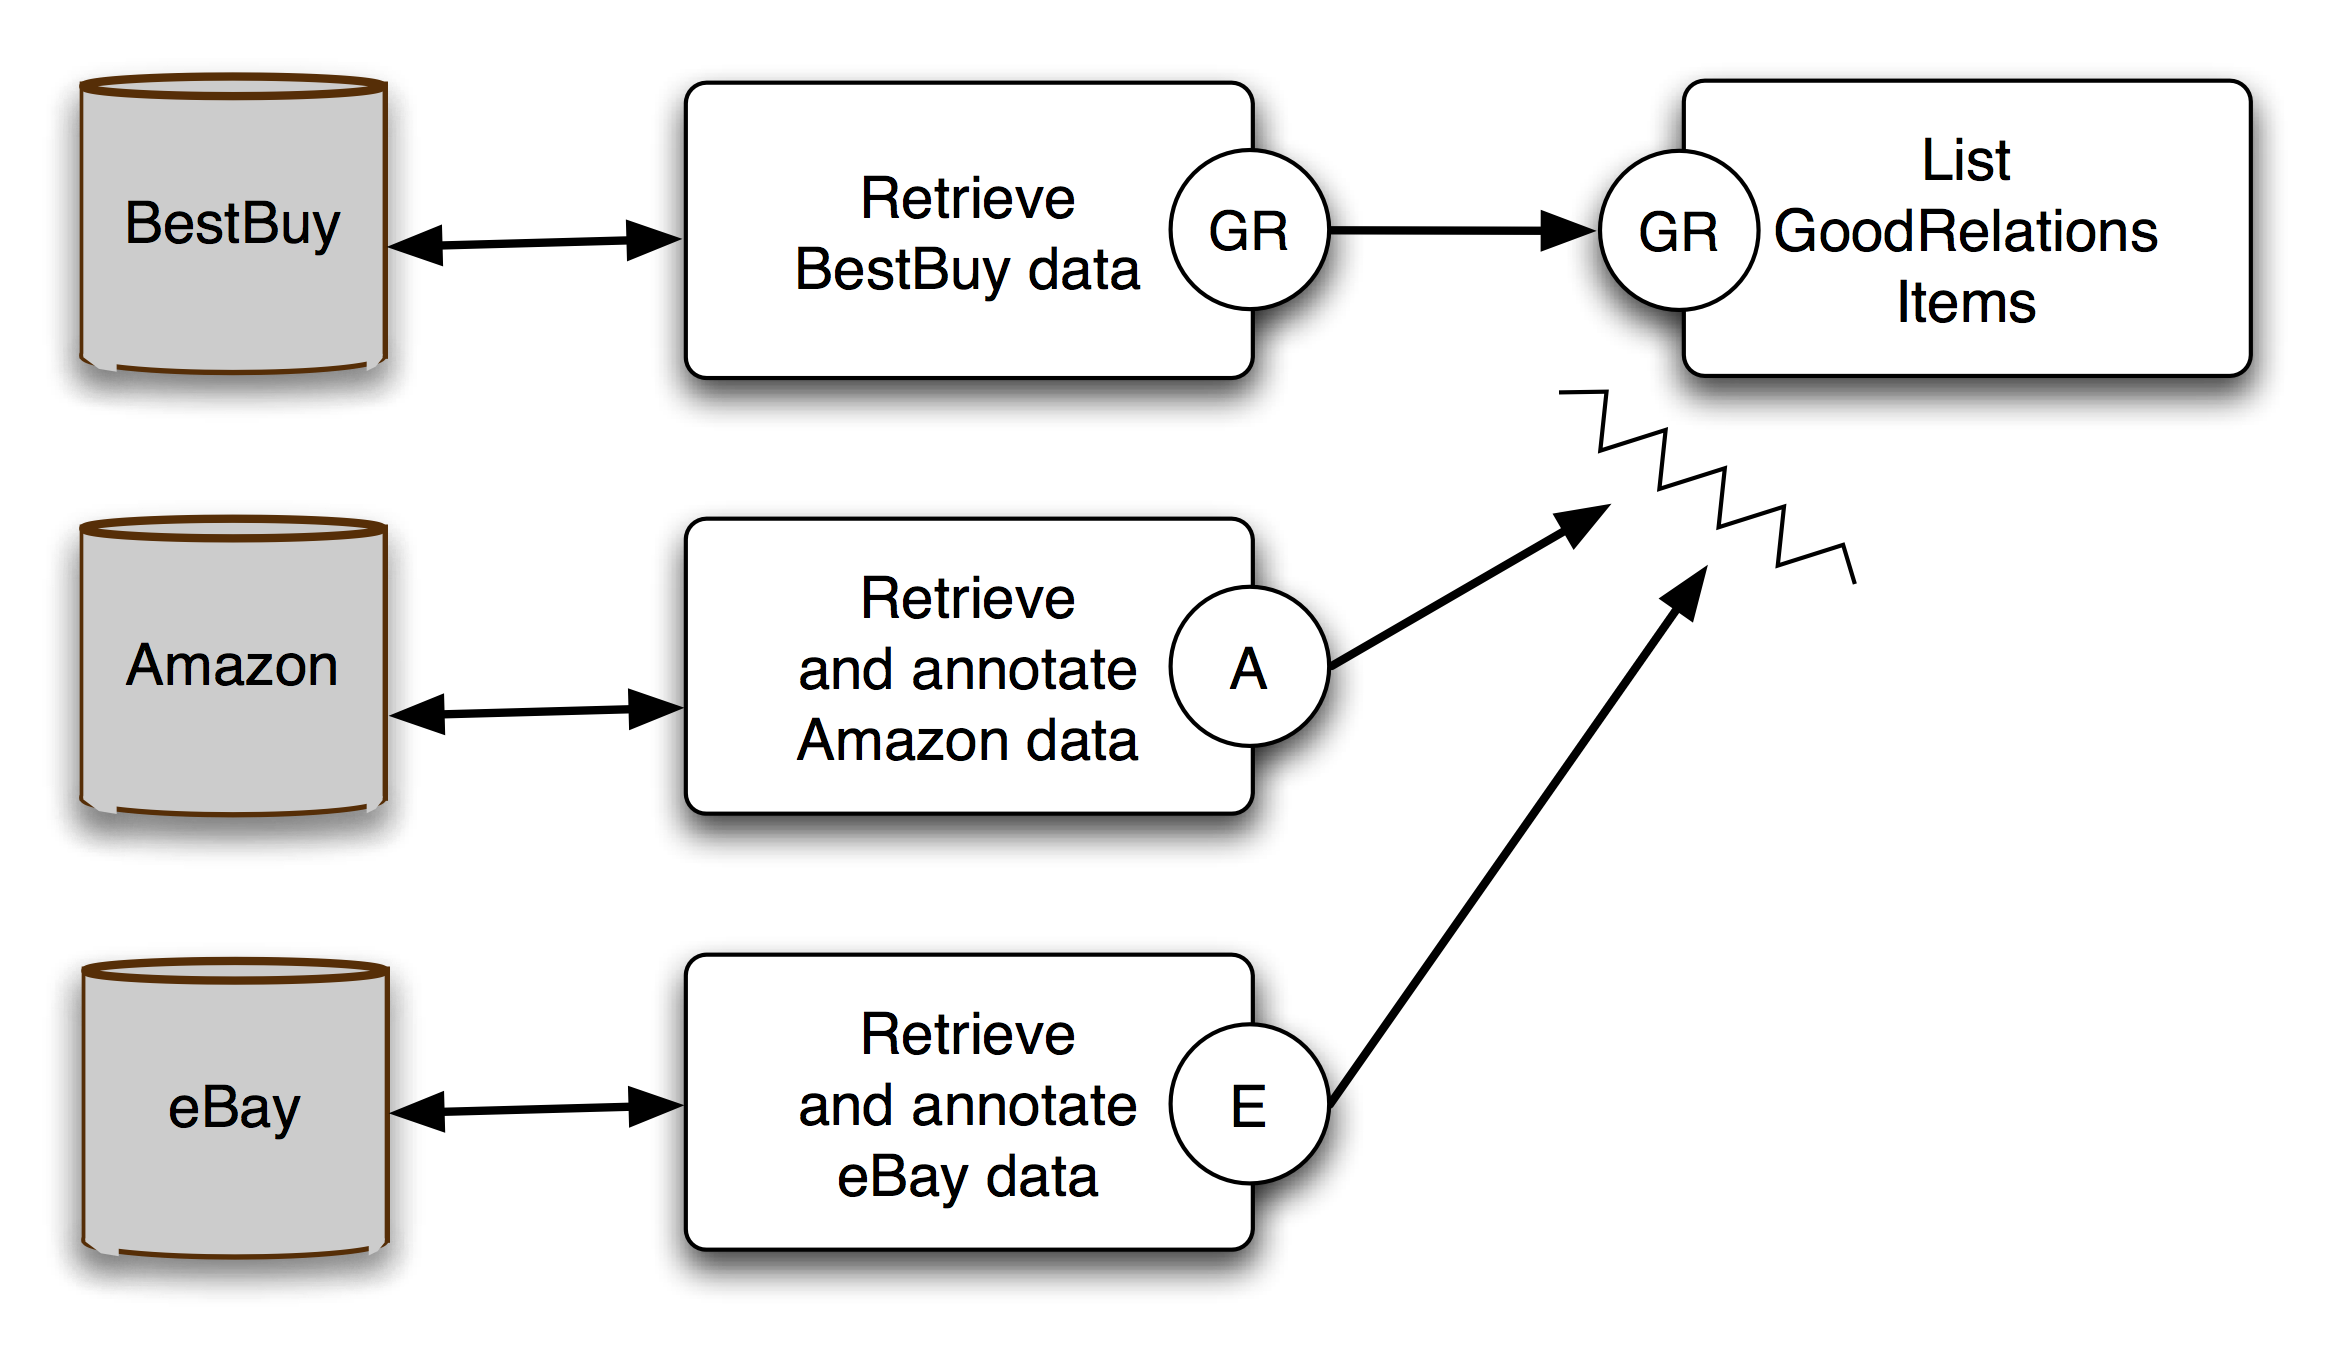
\includegraphics[width=8cm]{images/screens_diagram.png}%[bb=0 0 201 126]
        \caption{Three gadget components retrieving incompatible data}
    \label{fig:screens}
\end{figure}

Figure~\ref{fig:screens} illustrates our scenario. There are three retrieval components that wrap the different e-commerce sites and provide data according to three different ontologies: the GR ontology, the Amazon ontology (A) and the eBay ontology (E). Another component displays GR items for display to the user, but not A or E items. If the gadget designer wants to aggregate data from all three services in the display, there will therefore have to be a mapping present between A and E on the one hand, and GR on the other.

%, say we have a component that accesses the BestBuy service and retrieves RDF data that uses the GoodRelations ontology. In other words, the output of this component is GoodRelations data. Another component takes this data and displays them in a list, i.e. this component only accepts GoodRelations data for display. Since both components use the same ontology, they can be combined. However, now suppose we have two additional components, which access the Amazon and eBay services and retrieve items from there, which are then represented using the Amazon and eBay ontologies, respecitvely. The user wants to list items from all three sources in the same display component. However, since all three ontologies are incompatible, this is not possible out of the box. What is necessary is a mapping between the Amazon and GoodRelations, as well as eBay and GoodRelations ontologies.

%We have thus a case, where we want to aggregate data using three different ontologies, so aligning them to a common ontology is the only possible solution.

\subsection{Ontologies}
\label{ontologies}
Of the three ontologies used in our evaluation, only GoodRelations is a real-world, extensive ontology for e-commerce. The other two, i.e., the Amazon and the eBay ontologies were developed for simulation purposes as simplified versions of what would be used in the real-life scenarios. They were designed to showcase particular features of ontology mapping in our scenario.

\paragraph{GoodRelations:}
This ontology is aimed at annotating so-called ``offerings'' on the Web, which can be products or services. The ontology features support for ranges of units, measurements, currencies,  shipping and payments, common business functions (sell, lease, repair, etc.) and international standards (ISO 4217 or UNSPSC) and codes (e.g., EAN or UPC) in the field.
The main class is \texttt{Offering},
which represents an announcement by a \texttt{BusinessEntity} to provide a \texttt{ProductOrService} with a given \texttt{BusinessFunction}. It may be constrained in terms of eligible business partner, countries, quantities, and other properties. It is also described by a given \texttt{PriceSpecification}. The super-class for all classes describing products or service types is \texttt{ProductOrService}. This top-level concept has sub-classes representing actual product instances, product models and dummy product placeholders. A product is described by its title and description, manufacturer, make and model, etc. 
% While GoodRelations offers terminology to allow a much higher expressivity, we will restrict the discussion to those terms relevant for our scenario.


% \begin{center}
% \lstset{captionpos=b, breaklines=true}
% \lstset{frame=single, basicstyle=\scriptsize}
% \lstset{caption=Basic GoodRelations data in N3 notation, label=listing_gr}
% \lstset{language=XML}
% \begin{lstlisting}
% :Offering_8794691     a gr:Offering;
%   gr:hasPriceSpecification 
%       :UnitPriceSpecification_8794691_1;
%   gr:includesObject :TypeAndQuantityNode_8794691_1;
% 
% :UnitPriceSpecification_8794691_1     a gr:UnitPriceSpecification;
%   gr:hasCurrency "USD"^^xsd:string;
%   gr:hasCurrencyValue "749.99"^^xsd:float;
%   gr:hasUnitOfMeasurement "C62"^^xsd:string;
% 
% :TypeAndQuantityNode_8794691_1     a gr:TypeAndQuantityNode;
%   gr:amountOfThisGood "1.0"^^xsd:float;
%   gr:hasUnitOfMeasurement "C62"^^xsd:string;
%   gr:typeOfGood :ProductOrServicesSomeInstancesPlaceholder_8794691 .
% 
% :ProductOrServicesSomeInstancesPlaceholder_8794691 a gr:ProductOrServicesSomeInstancesPlaceholder;
%   gr:hasEAN_UCC-13 "0013803096095"^^xsd:string;
%   gr:hasMakeAndModel :PoSM_8794691;
%   rdfs:comment "With Auto Optimization and [...]"@en;
% 
% :PoSM_8794691     a gr:ProductOrServiceModel;
%   gr:hasManufacturer <bbuy:Manufacturer_Canon>;
%   rdfs:label "Canon EOS Digital Rebel [...]"@en;
%   rdfs:comment "With Auto Optimization and [...]"@en;
% \end{lstlisting}
% \end{center}


\paragraph{Amazon Ontology:}
We have created a small Amazon ontology based on a subset of the datatypes supported by the web service exposed by Amazon to third-party agents. The ontology describes \texttt{Items} based on the \texttt{ItemAttributes} description given in the Amazon Product Advertising API documentation\footnote{\url{http://docs.amazonwebservices.com/AWSECommerceService/latest/DG/}}.
The ontology features three classes for describing a product. Example instance data is given in List.~\ref{listing_amazon}.
\begin{inparaenum}[(1)]
    \item \texttt{Item} represents an Amazon item, defined by a title, a manufacturer, a product group (DVD, Book, etc.), an international EAN code, an ASIN (unique Amazon id), an author (for books) and a \texttt{ListPrice}. 
    \item \texttt{Company}, described by a  legal name, is used for representing the manufacturer of an \texttt{Item}.
    \item \texttt{ListPrice} has two properties: \texttt{hasCurrencyCode}, representing an ISO 4217 currency code (e.g. GBP or EUR), and \texttt{hasAmount} representing the price in the given currency.
\end{inparaenum}


% \begin{figure}[ht]
\lstset{caption=Simplified Amazon ontology data in N3 notation, label=listing_amazon}
\lstset{language=turtle}
\begin{lstlisting}
:Item_7590645 a amzn:Item;
   amzn:hasASIN "B0012YA85A";
   amzn:hasManufacturer :Manufacturer_Canon;
   amzn:hasModel "XSI Kit";
   amzn:hasPrice :Price_7590645_1;
   amzn:hasProductGroup "Electronics";
   amzn:hasTitle "Canon Digital Rebel XSi [...]" .
:Manufacturer_Canon a amzn:Company;
   amzn:hasLegalName "Canon" .
:Price_7590645_1 a amzn:ListPrice;
   amzn:hasAmount "575.55";
   amzn:hasCurrencyCode "GBP" .
\end{lstlisting}
% \end{figure}

\paragraph{eBay Ontology:}
The eBay ontology was created based on the eBay Shopping API\footnote{\url{http://developer.ebay.com/DevZone/shopping/docs/CallRef/index.html}} and is supposed to annotate data retrieved through the web service described by the API.
% \begin{center}
% \lstset{captionpos=b, breaklines=true}
% \lstset{frame=single, basicstyle=\small}
% \lstset{caption=Simplified eBay ontology data in N3 notation, label=listing_ebay}
% \lstset{language=XML}
% \begin{lstlisting}
% 
% :SimpleItem_1320648     a ebay:SimpleItem;
%   ebay:hasItemID "E012Y090912";
%   ebay:hasBidCount :"4";
%   ebay:hasCountry "UK";
%   ebay:hasCurrentPrice :Price_1320648_1;
%   ebay:hasPrimaryCategoryName "Electronics";
%   ebay:hasTitle "Canon Digital Rebel XSi [...]" .
%   ebay:hasDescription "Camera is practically unused. It's like new."
% 
% :Price_1320648_1     a ebay:CurrentPrice;
%   ebay:hasAmount "575.55";
%   ebay:hasAmountType "GBP" 
% \end{lstlisting}
% \end{center}
The ontology features three basic classes,
%  (see Listing \ref{listing_ebay} for an example of ebay data)
\begin{inparaenum}[(1)]
    \item \texttt{SimpleItem} represents an eBay \texttt{Item}, that is sold by a \texttt{SimpleUser}. It is described by a title, a \texttt{CurrentPrice} (specifying the highest bid, or the selling price of fix-priced items), primary category name, manufacturer, model, EAN code, item ID (a unique eBay ID), bid count, end time of bid, country where the item is located, and a product ID (which supports major international product codes --- this property is from the Finding API).
    \item The \texttt{CurrentPrice} features a \texttt{hasAmountType} property, specifying the currency code, and a \texttt{hasAmount} property, which is the amount of money for a price per unit.
    \item \texttt{SimpleUser} contains information about eBay users. Users are described by a user ID, about me URL and the seller's positive feedback score. This class will not be used for capturing information on goods for our scenario, but is an essential component of the eBay system, which was the reason for its inclusion in the ontology.
\end{inparaenum}

\subsection{Testing and Results}
\label{testing}

We present the approach an ontology engineer has to take to discover and represent ontology mappings, and a means to exploit them after the they have been discovered and appropriately represented.

There is a major paradigm difference between the GoodRelations ontology and the other two ontologies (see Sect.~\ref{sub:manual_mapping} for details). After some initial testing, we concluded that automatic mapping from GR to A/E using the string-based methods employed by the Alignment API tool was not feasible. Therefore, the following sections report on \emph{automatic mapping} for the A--E pair --- which are similar enough to be suitable for level 0 mapping ---, and \emph{manual mapping} for the GR--A/E pairs.

\subsubsection{Automatic Mapping}
\label{subsubsec:automaticmapping}

% \paragraph{The Matcher} % (fold)
% \label{par:the_matcher}

% paragraph the_matcher (end)
For automatic mapping of level 0 mappings, we used a simple string distance-based algorithm provided by Alignment API~\cite{euzenat2004api}, which computes the string distance between the names of the entities to find correspondences between them. Four methods have been used for computing the distance:
\begin{inparaenum}[(1)]
    \item equality, which tests whether the names are identical, 
    \item Levenshtein distance (number of character operations needed), 
    \item SMOA distance (which is a specialised distance for matching ontology identifiers) and
    \item a Wordnet-based~\cite{fellbaum1998wordnet} distance using the JWNL library with Wordnet.
\end{inparaenum}

The alignment description derived from these methods is given based on a simple vocabulary, containing a pair of ontologies and a set of correspondences, which express relations between entities of the two ontologies.
We used the level 0 mapping representation for representing simple mappings, which map discrete entities of the two ontologies. Thus the representation of the correspondences is given with the five elements described (with the \texttt{id} being optional), as shown in List.~\ref{listing_correspondence}. Similar mappings were were also used for more complex, manually-created representations (level 2), as detailed in Sect.~\ref{sub:manual_mapping}.

% \begin{figure}[ht]
% \begin{minipage}{\linewidth}
\lstset{caption=Level 0 mapping element example, label=listing_correspondence}
\lstset{language=turtle}
\begin{lstlisting}
<level_0_mapping> a align:Cell;
  align:entity1 amzn:hasCurrencyCode;
  align:entity2 ebay:hasAmountType;
  align:measure "1.0"^^xsd:float;
  align:relation "=" .
\end{lstlisting}
% \end{minipage}
% \end{figure}

% \subsubsection{Using the Tool.}
% The Alignment API tool can be used through a GUI, as a server or from the
% command-line interface, of which we have chosen the last one.
% The tool reads two RDF/OWL ontologies, computes the alignment between them, 
% performs some thresholding and displays the results. It can render the output
% in a number of formats, including HTML and XSLT.
% 
% An additional feature of the tool is its ability to evaluate results based on
% a reference alignment, and output the evaluation results in a table,
% or plot them as \LaTeX{} graphs.

\paragraph{Testing Procedure}
For the Amazon--eBay pair we set up a reference alignment, against which the results are evaluated.
We then ran the matching process for all for methods:
\begin{inparaenum}[(1)]
    \item equality,
    \item Levenshtein distance with a confidence threshold of \texttt{0.33} (meaning that any correspondence having a smaller confidence measure will be excluded),
    \item SMOA distance with a threshold of \texttt{0.5} and
    \item Wordnet distance using a threshold of \texttt{0.5}\footnote{Thresholds were selected based on suggestions in the Alignment API documentation}.
\end{inparaenum}
To apply the results, we rendered an XSLT template to transform an example dataset.

\paragraph{Results}

The results of automatically aligning the Amazon and eBay ontologies were quite favourable. As shown in Tab.~\ref{table_results}, we captured the four main parameters used in information retrieval, as described in \cite{olson2008advanced}. These four parameters are used for evaluating the performance of the alignment methods: 
\begin{inparaenum}[(1)]
    \item \textit{Precision}, the fraction of results that are correct --- the higher, the better, 
    \item \textit{Recall}, the ratio of the correct results to the total number of correct correspondences --- the higher, the better, 
    \item \emph{Fallout}, the fraction of incorrect results - the lower the better, and 
    \item \emph{F-measure}, which measures the overall effectiveness of the retrieval by a harmonic mean of precision and recall --- the higher, the better.
\end{inparaenum}

\begin{table}
    \centering
    \caption{Alignment results: Precision, Recall, Fallout and F-Measure}
    \label{table_results}

    \begin{tabular}{rrrrr}
        \toprule
        & \textbf{precision} & \textbf{recall} & \textbf{fallout} & \textbf{f-measure}\\
        \midrule
        \textbf{reference} & 1.00 & 1.00 & 0.00 & 1.00\\
        \textbf{equality} & 1.00 & 0.38 & 0.00 & 0.55\\
        \textbf{SMOA} & 0.43 & 0.75 & 0.57 & 0.55\\
        \textbf{Levenshtein} & 0.40 & 0.75 & 0.60 & 0.52\\
        \textbf{JWNL} & 0.67 & 0.75 & 0.33 & 0.71\\
        \bottomrule
    \end{tabular}
\end{table}

The first row (reference) shows the reference alignment, which, naturally, has both perfect precision and recall. We can observe what intuition has predicted, namely that pure string equality on term labels is far too simple and therefore irrelevant. By using string distances and giving certain thresholds (``Levenshtein and SMOA''), we can see that the results are much less precise, but have a better recall, since this allows for entities having similar names to be discovered, at the expense of having quite a few incorrect results; the thresholds allow for low-scored cases to be eliminated, although this results in the exclusion of some correct correspondences. The last row (``JWNL'') contains the results of the Wordnet-enabled method, which shows quite an improvement (precision of 0.67 and a recall of 0.75),
% \footnote{The scores are orientative, giving a general picture of how the process approaches 100\% efficiency}
due to the lexical analysis, which performs a much more relevant comparison of strings, giving a high number of correct results. The precision of the JWNL alignment shows only a tiny drop below the recall value, meaning that the number of incorrect correspondences discovered is small, and the main source of error is from the number of correspondences not discovered.


% \begin{center}
% \begin{figure}
% %% Plot generated by GenPlot of alignapi
% \begin{center}
% \begin{tikzpicture}[cap=round, scale=0.75]
% % Draw grid
% \draw[step=1cm,very thin,color=gray] (-0.2,-0.2) grid (10.0,9.0);
% \draw[|-|] (-0,0) -- (10,0);
% %\draw[dashed,very thin] (0,0) -- (5,8.66) -- (10,0);
% \draw[dashed,very thin] (10,0) arc (0:60:10cm);
% \draw[dashed,very thin] (0,0) arc (180:120:10cm);
% \draw (0,-0.3) node {$precision$};
% \draw (10,-0.3) node {$recall$};
% % Plots
% \draw plot[mark=+,] coordinates {(5.0,8.660254037844386)};
% \draw (5.01,8.370254037844385) node[anchor=south west] {Reference};
% \draw plot[mark=+,] coordinates {(9.296875,3.6834922606644636)};
% \draw (9.306875,3.3934922606644633) node[anchor=south west] {Equal};
% \draw plot[mark=+,] coordinates {(3.1058673469387754,2.9531229168449795)};
% \draw (3.115867346938775,2.6631229168449793) node[anchor=south west] {SMOA0.5};
% \draw plot[mark=+,] coordinates {(2.9875000000000003,2.6598578439458005)};
% \draw (2.9975,2.3698578439458003) node[anchor=south west] {Levenshtein0.33};
% \draw plot[mark=+,] coordinates {(4.409722222222222,4.99987943527481)};
% \draw (4.419722222222222,4.70987943527481) node[anchor=south west] {JWNL};
% 
% \end{tikzpicture}
% \end{center}
% \caption{Comparison of the four methods, against the reference alignment,\newline
% showing the distances from 0 precision and 0 recall}
% \label{fig:figure_alignment}
% \end{figure}
% \end{center}


We can deduce that the results provided are satisfactory, even though the methods used were simple, string-based ones, and the process was completely automated without any user input.
We are therefore confident that through some user assistance or an initial input alignment the tool can achieve 100\% correct results, which is our aim for the tool to be used in practice.


% \paragraph{XSLT:}
% One of the appealing features of the Alignment API is that it can render the results in XSLT, thus specifying a set of rules which make it possible to transform an  XML file from one format to the other. We have generated such an XML transformation description, and with the simple Linux application \texttt{xsltproc} (run from the command line) we have managed to transform data (limited, of course by the incompleteness of the alignment) from the Amazon ontology into data annotated by the eBay vocabulary. 
%Please refer to Appendix A for a listing of an example transformation.

\subsubsection{Manual Mapping} % (fold)
\label{sub:manual_mapping}

The GoodRelations ontology employs a unique paradigm, different from the paradigms of Amazon and eBay. In GR everything is centred around an instance of \texttt{Offering} and a graph of other instances attached to it, whereas for Amazon (and similarly for eBay), the main class is \texttt{Item}, which holds all relevant properties. In principle, \texttt{Item} would correspond to \texttt{ProductOrService} in GoodRelations, but the properties of the \texttt{Item} class are reflected as properties of many different classes in GR. 

Though the infeasibility of automating this alignment became obvious, we have represented the alignment in the mapping language supported by the tool, as a level 2 mapping (described in Sect.~\ref{mediation}).
 % (the mapping has been created between Amazon and GoodRelations, since the eBay and Amazon ontologies are very similar in approach, and mapping eBay to GoodRelations would be an indentical task). 
This mapping description can later be used by the run-time gadget code. List.~\ref{listing_gr_a} shows an example mapping between two properties of the two ontologies, specifying that the relationship is \texttt{Equivalence} with a certainty degree of \texttt{1.0}. This fragment does not show, but assumes the equivalence correspondence between the classes \texttt{Item} and \texttt{Offering}, which is a trivial level 0 mapping. This mapping specifies the relation

\begin{equation*} \label{eq}
\begin{split}
\forall{v,z}; hasEAN(v,z) & \Longrightarrow \exists{x, y}; includesObject(v,x) \wedge \\
&typeOfGood(x,y) \wedge hasEAN\_UCC\_13(y,z),
\end{split}
\end{equation*}

meaning that the \texttt{hasEAN} property of \texttt{v} in the Amazon ontology corresponds to the \texttt{hasEAN\_UCC\_13} property of the \texttt{typeOfGood} of the \texttt{includesObject} of \texttt{v} in GoodRelations. The domains and ranges of the properties are inferred, thus it is deduced, that in \texttt{Amazon v} is of type \texttt{Item} and \texttt{z} is \texttt{int}, and in \texttt{GoodRelations v, x, y} and \texttt{z} are instances of the classes \texttt{Offering}, \texttt{TypeAndQuantityNode}, \texttt{ProductOrService} and \texttt{int}, respectively.

\begin{figure}[ht]
\lstset{caption=Fragment of the Amazon--GoodRelations mapping, label=listing_gr_a}
\lstset{language=turtle}
\begin{lstlisting}
<level_2_mapping> a align:Cell;
   align:entity1 amzn:hasEAN;
   align:entity2 
      [ a align:Property;
        align:first gr:includesObject;
        align:next gr:hasEAN_UCC_13,
           gr:typeOfGood ];
     align:measure "1.0"^^xsd:float;
     align:relation "Equivalence" .

amzn:hasEAN a align:Property .
gr:hasEAN_UCC_13 a align:Property .
gr:includesObject a align:Relation .
gr:typeOfGood a align:Relation .
\end{lstlisting}
\end{figure}

% \begin{center}
% \lstset{caption=Fragment of the Amazon--GoodRelations mapping, label=listing_gr_a}
% \lstset{language=xml}
% \begin{lstlisting}
% <Cell rdf:about="MappingRule_01">
%  <entity1><omwg:Property rdf:about="&amzn;hasEAN"/></entity1>
%  <entity2>
%   <omwg:Property>
%     <first><Relation rdf:about="&gr;includesObject"/></first>
%     <next><Relation rdf:about="&gr;typeOfGood"/></next>
%     <next><Property rdf:about="&gr;hasEAN_UCC_13"/></next>
%   </omwg:Property>
%  </entity2>
%  <measure rdf:datatype="&xsd;float">1.0</measure>
%  <relation>Equivalence</relation>
% </Cell>
% \end{lstlisting}
% \end{center}

Using this representation, complex correspondences can be modelled, using first order logic constructs.

\subsection{Fact Transformation Tool}
\label{sec:fact_tool}

To support the application of previously created mapping rules, we have developed a rule based, interactive \emph{fact transformation tool} (or \emph{fact tool} for short). This tool utilises techniques of our service wrapper tool. One part of the service wrapper tool~\cite{rivera2011connecting} uses a rule-based approach for the transformation of web service responses into FAST facts (i.e., instances of ontology concepts). The application of ontology mediation rules can be modelled in a similar vein. In the fact tool, we therefore use analogous rule-based techniques to create data transformation operators, i.e., operators that mediate between two different conceptualisation.

\begin{figure}
    \centering
    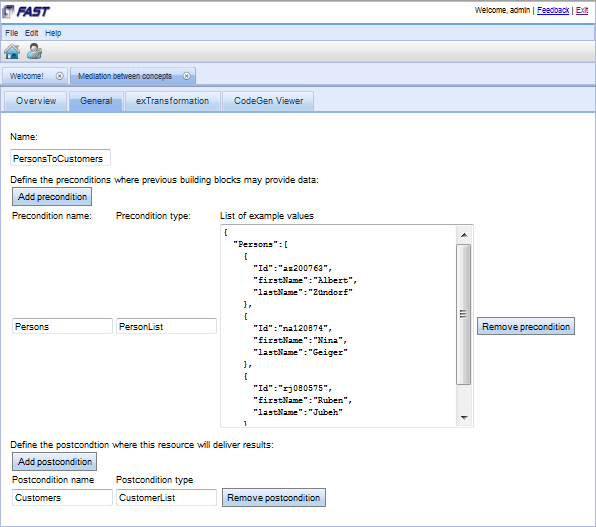
\includegraphics[width=0.8\linewidth]{images/GVSMediationToolPreconditions.png}
    \caption{Definition of operator pre- / postconditions}
    \label{fig:FactsTransformationToolPortDefinitions}
\end{figure}

Figure \ref{fig:FactsTransformationToolPortDefinitions} shows a screen shot of the  fact transformation tool within the GVS environment. The tool has four tabs\footnote{The \texttt{CodeGen Viewer} tab is explained later in Sect.~\ref{sec:runtime}.}, of which the \textit{General} tab (currently shown in the screen shot) is employed to define the pre- and postconditions for the desired data transformation operator in a first general step. 
Using the terminology introduced previously, this allows to define a basic \emph{level 0} mapping between two concepts (\texttt{PersonList} and \texttt{CustomerList} in the example).
The fact tool communicates with the FAST catalogue to select concepts and provide example instances (as JSON data structures) that help the user to perform the correct choice.
% These conditions are typed according to the participating semantic elements to be derived from the FAST catalogue. This typing will provide the structure of the input and output data of the desired data transformation operator.  
After this step, the mapping can be refined to a higher level by defining concrete transformation rules. These can be edited in the \emph{exTransformation} tab as shown in Fig.~\ref{fig:FactsTransformationToolTransformationRules}. On the left of the tab the user is presented with a tree of example data for the input concept, while the right side of the tab shows a similar tree with the derived data for the output concept. This way, the user can continuously observe the effect of changes in the rule they are currently editing. The fact tool constantly executes the transformation rules after any editing, giving direct feedback on their effect and thus enabling the user to validate the achieved transformation. 

\begin{figure}
  \begin{center}
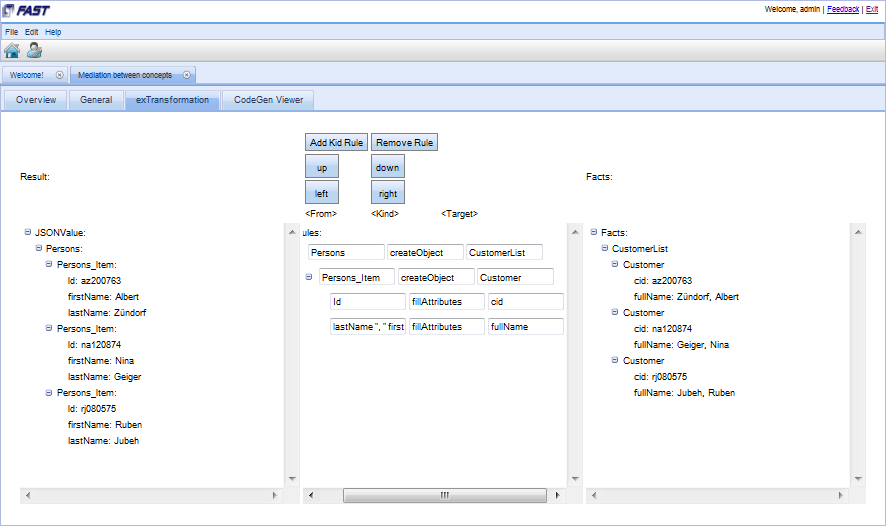
\includegraphics[width=\linewidth]{images/FactsTransformationToolGVSWithTransformationRules.png}
    \caption{Interactive, rule-based transformation of Person facts}
    \label{fig:FactsTransformationToolTransformationRules}
  \end{center}
\end{figure}

Examples for the rules themselves are shown in the rule tree in the middle of Fig.~\ref{fig:FactsTransformationToolTransformationRules}. Starting with a root rule, additional rules can be added as child-rules, while existing rules can be moved around the tree or deleted. Rules can have different types, such as \emph{createObject} or \emph{fillAttributes}. A \textit{createObject} rule can be used to create output fact objects. The \textit{Target} field of such a rule specifies the type of the created objects (i.e., a concept from the FAST catalogue), in our example \textit{List}. The top rule fires for each element of the input data with the type specified in the \textit{From} field of the transformation rule. Thus, in our example, the input data is searched for objects of type \textit{List} firing for the root of our data. The second rule of our example creates \textit{Customer} objects. This rule is a sub-rule of the root rule and thus the created objects are added to the \textit{List} object created by the parent rule. Similarly, the search for triggering objects of type \textit{Person} is restricted to the subtree below the from element that has triggered the parent rule, i.e. to our input \textit{List}. The third rule is used to fill the attribute \textit{fullName} of the \textit{Customer} objects. This rule is an example for a many-to-one transformation. The result is a string concatenation of the \textit{lastName} of the \textit{Person} that has triggered the parent rule plus a text constant plus the \textit{firstName} of the current \textit{Person}. The resulting string is transferred to the \textit{fullName} attribute of the corresponding \textit{Customer}. 

Note that simple one-to-one transformation rules may be derived with the help of the ontology mediation approach described in Sect.~\ref{subsubsec:automaticmapping}. Such simple rules can be added to the transformation tool, automatically. The more complex rules may then be added interactively. During editing, the semantics provided by the FAST catalogue are used to support the user with completion proposals and consistency checking. In addition, the direct execution of the rules on example data helps the user to create appropriate rules and to validate their effects. 

So far our transformation rules are restricted to simple cases. We have focused on simple cases allowing a simple transformation approach that does not require sophisticated skills from our users. 


\subsection{Creating the Operator}
\label{sec:creating_the_operator}

Once the data transformation operator has been defined, it may be added to the FAST catalogue in order to allow its use for the definition of piping configurations of new screens within the FAST GVS tool. For this purpose a simple semantic description is sent to the FAST catalogue defining the semantics of the operator and the semantics of its pre- and postconditions. This is shown in Fig.~\ref{fig:operator_in_screen_builder}, where the newly created data transformator for mediating between Person and Customer concepts (i.e., transforming instances of one concepts into instances of the other) has been saved and is now available in the GVS screen builder interface as an filter operator. 

\begin{figure}[h]
  \begin{center}
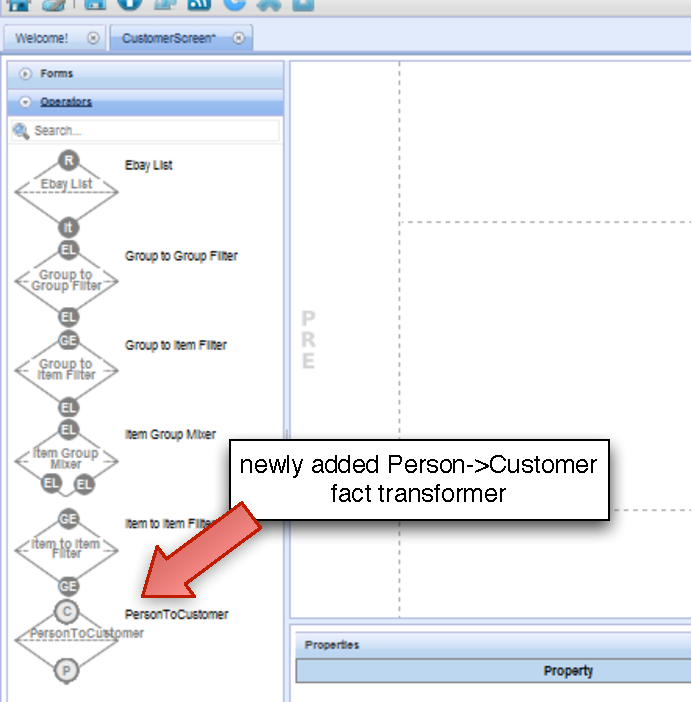
\includegraphics[width=.6\linewidth]{images/operator_closeup}
    \caption{A newly created operator in the GVS screen builder}
    \label{fig:operator_in_screen_builder}
  \end{center}
\end{figure}

The Service Wrapper Tool uses its own repository for trees of transformation rules. First of all this has technical reasons: the development of the transformation tool is based on a reference architecture and libraries for web-based interactive systems provided by Kassel University~\cite{AsDH2009CVSM}. This repository has the special advantage that it provides support for teams of developers, thus the service wrapper tool allows to merge the contributions of multiple developers. 


\section{Gadget Building  and Runtime}

Neither gadget (or screenflow) building or runtime are directly involved with the ontology mapping process. However, the steps performed previously affect these phases of the lifecycle as well, as discussed briefly in the sections below.

\subsection{Gadget Building} % (fold)
\label{sec:gadgetbuilding}

Every time ontology matching is performed and an alignment is created between two underlying resources, the corresponding alignment rules are stored and an operator building block is created in the catalogue, to be available during screen development. 

During the gadget building phase, whenever pre- and post-conditions of screens, resources or operators show a semantic mismatch, the catalogue offers the possible matching operators that would solve the incompatibility problem. This way a matching operator can be placed between two pre- and postconditions that would otherwise be incompatible, making interoperation between the two possible. In seldom cases, the catalogue may fail to retrieve an appropriate mediation operator. In such cases, the possibility of building a new mapping operator with the help of the fact transformation tool is presented, allowing the user to assume the role of ontology engineer in special cases.  

\subsection{Runtime} 
\label{sec:runtime}
For deployment, the gadget's implementation is generated as an executable bundle containing a portion of Javascript code. In addition, a small FAST runtime library (again Javascript) is added to the gadget. This runtime library provides notification mechanisms and manages the fact base of the gadget. For data transformation purposes (i.e., ontology mapping) we generate Javascript code that connects itself to the fact base. Any time a fact is sent to the pre-condition of the operator, it performs the data transformation and sends the result to the post-condition. The code generated from the transformation rules follows a recursive pattern, where each rule is represented as a Javascript function with parameters for the source and target fact subtrees to be transformed. The function body then uses code to search the source tree for sub elements that match the \textit{From} part of the rule and then code for the desired operation is generated. For debugging purposes the user can examine the code generated for an operator in the \textit{CodeGen Viewer} tab of the fact tool. 

Our code generation for service wrappers and transformation operators uses a template-based approach. Thus, the \textit{CodeGen Viewer} tab will also allow to examine the templates used for code generation and to adapt the templates in order to meet changing APIs or to meet new requirements. Thereby, the code generation is not hard wired into our tool but may be adapted by (skilled) end users on the fly. 

\section{Summary}
\label{sec:summary}
With the Semantic Web winning more and more ground both in research and industry, the mismatches between ontologies used by the inter-operating systems present an increasing problem. Ontology matching deals with identifying these mismatches, and overcoming them. 

The initial work on the ontology matching comprised an overview of the area in general, and was reflected in the first iteration of this deliverable (\cite{ambrus2009mediation}, now in App.~\ref{sec:background}). In it, we discussed the theoretical foundations of ontology matching. After presenting the main problem and the types of mismatches between ontologies, we presented --- based on a study of the state-of-the-art in these areas --- the three main approaches to ontology mediation, i.e., \textit{ontology mapping} (representing  correspondences between entities), \textit{ontology alignment} (the process of finding the correspondences between ontologies) and \textit{ontology merging} (the process of creating a new ontology based on the source ontologies that need to be reconciled). 

The second iteration of the document~\cite{ambrus2010mediation} saw a positioning of ontology matching within the FAST project, both in terms of the FAST lifecycle and its associated user roles. It was defined which phases are affected in which way, and which actions by particular user roles are involved. We have shown how matching is done at the different phases of the gadget life cycle and the approach taken at every level. Additionally, we covered different candidates for tools to support automatic matching algorithms and evaluated the most promising ones on the backdrop of an e-commerce scenario. It was found that, while automatic matching is feasible for some, mostly simple cases, the manual definition of mapping rules will still be necessary for many real-life cases. Research into new methods for automatic matching of complex cases was deemed outside the scope of this project. Instead, the focus was on supporting users of the FAST tool to manually define mapping rules in an intuitive fashion. To this end, a first standalone prototype of the \emph{fact transformation tool} was developed and presented briefly.

This final iteration of the deliverable focussed mainly on the improvement of the fact tool and its transformation of a standalone tool into an integral part of the FAST tool chain, thereby supporting users and allowing them to use the same kind of interaction and user interface throughout the platform. The fact tool presented in this deliverable and the service wrapping tool presented in \cite{rivera2011connecting} therefore use a similar graphical approach. Without leaving the FAST platform, users can now assume the role of ontology engineer and define mapping rules of varying complexity, which can then be saved as operator building blocks, to be used in the screen development process. To allow this, the fact tool communicates with the FAST catalogue to guide users in the rule creation process and outputs definitions according to the FAST gadget ontology, as well as code to be used in the deployed gadget.

